\documentclass{scrartcl}
%\documentclass{article}
\usepackage[utf8]{inputenc}
\usepackage[T1]{fontenc}
\usepackage[ngerman]{babel}
\usepackage{amsmath}
\usepackage{amsthm}
\usepackage{graphicx}
%\usepackage{cite}

 
\title{Wintersemester 2013/2014 \\
  JAVA-Programmierpraktikum 1580 \\
  Thema: Kulami (Entwurf)
}
\author{Gordon Martin\\
  Matr.-Nr. 8038813 \\
  gordon.martin@fernuni-hagen.de
}

\date{17.11.2013}

\begin{document}
 
\maketitle
\thispagestyle{empty}

\pagenumbering{arabic} 
\setcounter{page}{1}


\section{Klassendiagramm}
\label{sec:Klassendiagramm}

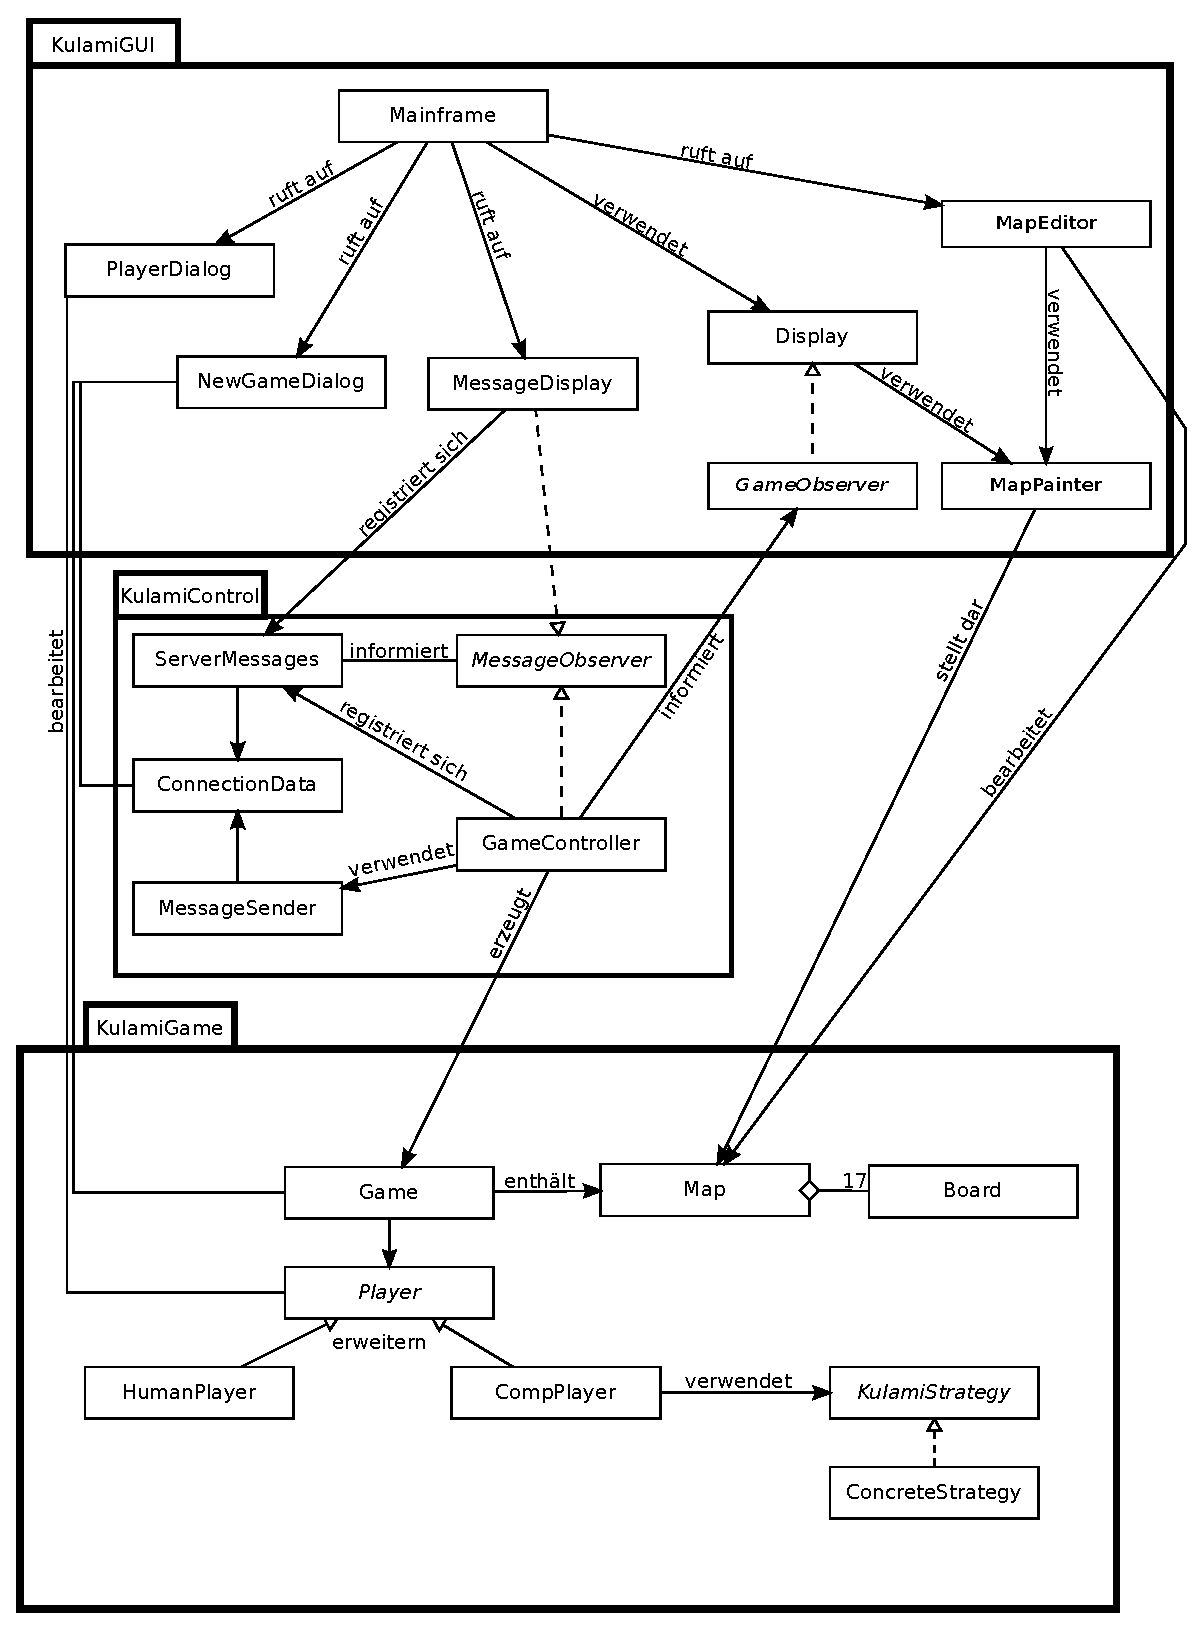
\includegraphics[width=15cm]{../docs/KulamiKlassendiagramm_Inkscape}

\section{Funktionalität der Klassen}
\label{sec:Funktionalitaet}

Der Übersichtlichkeit halber ist das Programm in drei Pakete aufgeteilt: KulamiGame, KulamiControl und KulamiGUI.

\subsection{KulamiGame}
\label{sec:Spielklassen}

Die Klassen in diesem Paket repräsentieren ein Kulamispiel mit einem Spielfeld und einem Spieler.


\subsubsection{Game}
\label{sec:Game}

\texttt{Game} enthält das aktuelle Spiel und den Spielstand. Dazu enthält \texttt{Game} das Spielfeld, die aktuelle Belegung des Spielfeldes und Informationen zu den Spielern.  \texttt{Game} enhält Methoden, die Informationen zum Spielstand liefern:

\begin{itemize}
\item letzter Zug
\item vorletzter Zug
\item zulässige Felder für den aktuellen Zug
\item Plattenbesitz für jeden Spieler
\item Punktestand für jeden Spieler
\end{itemize}

Außerdem enthält \texttt{Game} Methoden, um den Zustand des Spiels zu manipulieren und einen neuen Spielstand zu erzeugen:

\begin{itemize}
\item platziere Murmel
\item breche Spiel ab
\end{itemize}

\subsubsection{Player}
\label{sec:Player}

\texttt{Player} ist eine abstrakte Klasse, die einen Spieler repräsentiert. Ein \texttt{Player} kann Murmeln platzieren und das Spiel abbrechen.

\subsubsection{HumanPlayer}
\label{sec:HumanPlayer}

\texttt{HumanPlayer} repräsentiert einen menschlichen Spieler. Ein menschlicher Spieler kann Murmeln platzieren und das Spiel abbrechen.  Ein \texttt{HumanPlayer} hat einen Namen.

\subsubsection{CompPlayer}
\label{sec:CompPlayer}

\texttt{CompPlayer} wird im KI-Modus verwendet.  Ein \texttt{CompPlayer} ist ein automatischer Spieler, der selbständig Murmeln platziert.  Ein \texttt{CompPlayer} bricht das Spiel nicht ab.  Zur Auswahl des nächsten Zuges benötigt ein \texttt{CompPlayer} ein Objekt, das \texttt{KulamiStrategy} implementiert.

\subsubsection{KulamiStrategy}
\label{sec:KulamiStrategy}

\texttt{KulamiStrategy} ist ein Interface, das eine Methode fordert, die gegeben eines Spielstands den nächsten Zug liefert.  Eine \texttt{KulamiStrategy} wird parametrisiert mit einer Stufe von 1 bis 10.

\subsubsection{ConcreteStrategy}
\label{sec:ConcreteStrategy}

\texttt{ConcreteStrategy} ist eine Implementierung von \texttt{KulamiStrategy}.  Eine \texttt{ConcreteStrategy} liefert einen konkreten Algorithmus zur Auswahl des nächsten Zuges.  Es kann mehrere Implementierungen \texttt{ConcreteStrategy1}, \texttt{ConcreteStrategy2}, usw. geben, die zur Laufzeit ausgetauscht werden können.

\subsubsection{Map}
\label{sec:Map}

Die Klasse \texttt{Map} repräsentiert ein Spielfeld bestehend aus 17 Platten.  \texttt{Map} bietet Methoden zum Abfragen der Plattenkonfiguration und der Belegung sowie zum Platzieren einer Murmel an.

\subsubsection{Board}
\label{sec:Board}

Ein \texttt{Board} repräsentiert eine der 17 Platten eines Spielfeldes.

\subsection{KulamiControl}

KulamiControl enthält Klassen, die für den Ablauf des Spiels und die Kommunikation mit dem Spieleserver verantwortlich sind.

\subsubsection{GameController}
\label{sec:GameController}

Der \texttt{GameController} verwaltet den Ablauf des Spiels.  Er speichert Verbindungsdaten in einem \texttt{ConnectionData}-Objekt und erzeugt ein \texttt{ServerMessages}-Objekt zum Empfang von Servernachrichten und ein \texttt{MessageSender}-Objekt zum Versand von Nachrichten an den Server.  Der \texttt{GameController} implementiert das \texttt{MessageObserver}-Interface und registriert sich beim \texttt{ServerMessages}-Objekt als Nachrichtenempfänger.  Der \texttt{GameController} erzeugt außerdem ein \texttt{Game}-Objekt, in dem das aktuelle Spielrepräsentiert wird ist.


\subsubsection{ServerMessages}
\label{sec:ServerMessages}

\texttt{ServerMessages} empfängt in einer Endlosschleife Nachrichten vom Kulamiserver.  Die Verbindungsdaten sind in einem \texttt{ConnectionData}-Objekt enthalten.  Um den Programmablauf nicht zu blockieren, läuft \texttt{ServerMessages} in einem eigenen Thread.  Wenn eine neue Nachricht eingeht, informiert \texttt{ServerMessages} alle Objekte, die sich als \texttt{MessageObserver} registriert haben.

\subsubsection{MessageSender}
\label{sec:MessageSender}

\texttt{MessageSender} enthält Methoden zum Versenden von Nachrichten an den Kulamiserver.  Die Verbindungsdaten sind in einem \texttt{ConnectionData}-Objekt enhalten.

\subsubsection{ConnectionData}
\label{sec:ConnectionData}

\texttt{ConnectionData} enthält Verbindungsdaten zum Kulamiserver.

\subsubsection{MessageObserver}
\label{sec:MessageObserver}

\texttt{MessageObserver} ist ein Interface, das von allen Klassen implementiert werden muss, die von\texttt{ ServerMessages} über neue Servernachrichten informiert werden wollen.

\subsection{KulamiGUI}
\label{sec:GUI}

KulamiGUI enthält alle Klassen, die mit der Darstellung des Spiels zu tun haben.

\subsubsection{Mainframe}
\label{sec:Mainframe}

\texttt{Mainframe} ist die Hauptklasse für die GUI, die alle anderen Elemente enthält.  Der \texttt{Mainframe} enthält ein Spieldisplay, ruft Dialoge und den \texttt{MapEditor} auf und startet den \texttt{GameController}.

\subsubsection{Display}
\label{sec:Display}

Im \texttt{Display} wird der aktuelle Spielstand angezeigt.  \texttt{Display} verwendet \texttt{MapPainter}, um das aktuelle Spielfeld zu zeichnen.  \texttt{Display} implementiert \texttt{GameObserver}, um bei Änderungen des Spielstands informiert zu werden und sich zu aktualisieren.

\subsubsection{MapPainter}

\texttt{MapPainter} ist eine Hilfsklasse, die ein Spielfeld zeichnen kann.

\subsubsection{GameObserver}
\label{sec:GameObserver}

\texttt{GameObserver} ist ein Interface, das von Klassen implementiert wird, die über Änderungen des Spielstands informiert werden wollen.

\subsubsection{MapEditor}

Der \texttt{MapEditor} ist ein graphischer Editor, in dem Spielfelder erstellt und bearbeitet werden können.

\subsubsection{PlayerDialog}

Im \texttt{PlayerDialog} kann ein neuer Spieler erzeugt werden.

\subsubsection{NewGameDialog}

Mit dem \texttt{NewGameDialog} wird ein neues Spiel gestartet.  Für ein neues Spiel müssen eine Serverbindung (\texttt{ConnectionData}), ein Spieler (\texttt{Player}) und ein Spielfeld (\texttt{Map}) zur Verfügung stehen.  Im \texttt{NewGameDialog} gibt der Benutzer die Verbindungsdaten zum Kulamiserver an und wählt ein Spielfeld aus.

\subsubsection{MessageDisplay}

Im \texttt{MessageDisplay} werden Nachrichten für den Spieler angezeigt.  Dies können Mitteilungen des gegnerischen Spielers oder für den Spieler relevante Servernachrichten sein.  Um über Servernachrichten informiert zu werden, registriert sich \texttt{MessageDisplay} bei \texttt{ServerMessages} als \texttt{MessageObserver}.



\section{Beziehungen zwischen den Klassen}
\label{sec:Beziehungen}

Das Programm wird im \texttt{Mainframe} gestartet.  Der \texttt{Mainframe} startet den \texttt{GameController}.  Der \texttt{GameController} hat Assoziation zu allen drei Bereichen des Programms.  Damit ist \texttt{GameController} die eigentliche Hauptklasse, die die verschiedenen Komponenten miteinander verbindet.  Insbesondere verwaltet der \texttt{GameController} ein Objekt mit den Serververbindungsdaten und startet den Empfang vom und den Versand von Nachrichten an den Server.  Der \texttt{GameController} hat außerdem ein Modell des Spielzustands und informiert bei Änderungen des Spielzustands alle registrierten \texttt{GameObserver}, also das \texttt{Display}-Objekt, welches für die Darstellung des Spiels zuständig ist.

Das Spielzustandsmodell besteht aus der Klasse \texttt{Game} und den mit ihr verbundenen Klassen \texttt{Map} und \texttt{Player}.  \texttt{Map} repräsentiert das Spielfeld, bestehend aus 17 \texttt{Board}s.  \texttt{Game} speichert sowohl die verwendete \texttt{Map} als auch die \texttt{Map} mit der aktuellen Belegung.  \texttt{Player} ist eine abstrakte Klasse, die von \texttt{HumanPlayer} und \texttt{CompPlayer} erweitert wird.  Zu \texttt{CompPlayer} gehört eine \texttt{KulamiStrategy}, die als Interface verbunden ist, damit verschiedene konkrete Strategien ausprobiert werden können.

Die KulamiControl-Komponente enthält Klassen zur Kommunikation mit dem Spieleserver.  \texttt{ServerMessages} empfängt Nachrichten vom Server und informiert alle registrierten \texttt{MessageObserver}.  \texttt{MessageObserver} sind der \texttt{GameController}, der auf Nachrichten ggf. mit Änderungen des Spielzustands reagiert, und das \texttt{MessageDisplay}, das dem Benutzer relevante Nachrichten (z.B. Chatnachrichten)  anzeigt.  Eine Debuggingkonsole könnte auf die gleiche Art angeschlossen werden.  Der \texttt{MessageSender} sendet Nachrichten an den Server.

Die Benutzeroberfläche ist im \texttt{Mainframe} enthalten.  Die Klasse \texttt{Display} ist dafür zuständig, das aktuelle Spielfeld darzustellen.  Für das Zeichnen der Map wird eine eigene Klasse \texttt{MapPainter} verwendet.  \texttt{PlayerDialog}  ist zuständig für die Erstellung eines Spielerprofils.  Der \texttt{MapEditor} ist ein Editor zur Erstellung und Bearbeitung von Spielfeldern und verwendet ebenfalls \texttt{MapPainter} für die Darstellung des Spielfeldes.

Bevor ein Spiel gestartet werden kann, muss der Benutzer mit dem \texttt{PlayerDialog} einen Spieler anmelden.  Dann kann der Benutzer mit dem \texttt{NewGameDialog} die Verbindungsdaten zu einem Kulamiserver angeben und den Client mit dem Server verbinden.  Falls der Benutzer als erster Spieler einem Spiel beitritt, muss er ein Spielfeld auswählen.

\end{document}